\documentclass[11pt,letterpaper]{article}
\usepackage[utf8]{inputenc}
\usepackage[left=1in,right=1in,top=1in,bottom=1in]{geometry}
\usepackage{amsfonts,amsmath}
\usepackage{graphicx,float}
% -----------------------------------
\usepackage{hyperref}
\hypersetup{%
  colorlinks=true,
  linkcolor=blue,
  citecolor=blue,
  urlcolor=blue,
  linkbordercolor={0 0 1}
}
% -----------------------------------
\usepackage{fancyhdr}
\newcommand\course{MATH-UA.0252\\Numerical Analysis}
\newcommand\hwnumber{10}                  % <-- homework number
\newcommand\NetIDa{Ryan Sh\`iji\'e D\`u} 
\newcommand\NetIDb{November 18th, 2022}
\pagestyle{fancyplain}
\headheight 35pt
\lhead{\NetIDa\\\NetIDb}
\chead{\textbf{\Large Worksheet \hwnumber}}
\rhead{\course}
\lfoot{}
\cfoot{}
\rfoot{\small\thepage}
\headsep 1.5em
% -----------------------------------
\usepackage{titlesec}
\renewcommand\thesubsection{(\arabic{section}.\alph{subsection})}
\titleformat{\subsection}[runin]
        {\normalfont\bfseries}
        {\thesubsection}% the label and number
        {0.5em}% space between label/number and subsection title
        {}% formatting commands applied just to subsection title
        []% punctuation or other commands following subsection title
% -----------------------------------
\setlength{\parindent}{0.0in}
\setlength{\parskip}{0.1in}
% -----------------------------------
\input{../../command.tex}
\begin{document}

\section{Singular Value Decomposition (SVD) basics}
\subsection{}
Like QR, SVD has the full and reduced form \cite{TrefethenBau_97}:
\begin{figure}[H]
    \centering
    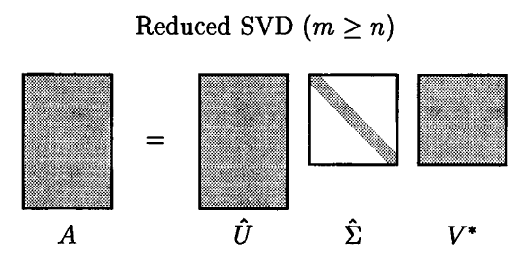
\includegraphics[width = 0.49\textwidth]{figs/TB_reducedSVD}
    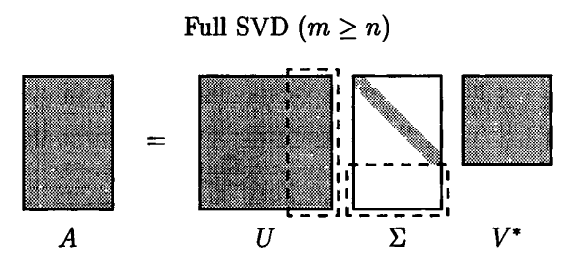
\includegraphics[width = 0.49\textwidth]{figs/TB_fullSVD}
\end{figure}
Note that the full form has $U$ which spans the whole of $\mathbb{R}^n$.

\subsection{}
We can interpret the full form of SVD as a change of basis, then a scaling, and then another change of basis (Figure from \cite{Strang_93}).
\begin{figure}[H]
    \centering
    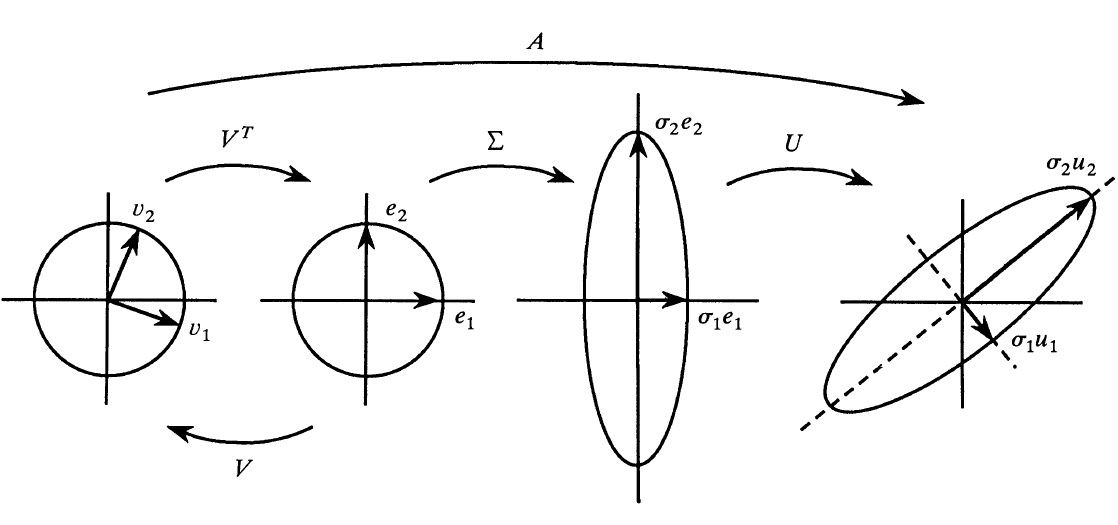
\includegraphics[width = 0.7\textwidth]{figs/strang_SVD}
\end{figure}

\section{Some properties of SVD}
We list (and attempt to prove) some properties of SVD:

\subsection{}
$\text{range}(A) = \text{span}(\ve u_1,\ve u_2,\dots,\ve u_r)$ and $\text{null}(A) = \text{span}(\ve v_{r+1},\dots,\ve v_n)$. 

\subsection{}
The rank of $A$ is $r$, the number of nonzero singular values.

\subsection{}
We have $\norm{A}_2 = \sigma_1$, the largest singular value. And $\norm{A}_F = \sqrt{\sigma_1^2+\sigma_2^2+\dots+\sigma_r^2}$. 

You will show the second property in your homework.

\section{Low-rang approximation using SVD}
\subsection{}
Show that $A$ is the sum of $r$ \emph{rank-one} matrices:
\begin{align*}
    A = \sum_{j=1}^r \sigma_j \ve u_j \ve v_j^\top.
\end{align*}

\subsection{}
For any $\nu$ with $0\leq \nu \leq r$, define
\begin{align*}
    A_\nu = \sum_{j=1}^\nu \sigma_j \ve u_j \ve v_j^\top.
\end{align*}
Then we have
\begin{align*}
    \norm{A-A_\nu}_2 = \inf_{\substack{B\in\mathbb{R}^{m\times n}\\\text{rank}(B)\leq\nu}}\norm{A-B}_2 = \sigma_{\nu+1}.
\end{align*}

Note that a similar theorem is also true for the Frobenius norm.

\section{Polynomial interpolation and linear algebra}
In lecture you have learned the theorem which states:

For $n\geq 1$ and distinct $n+1$ data pairs $(x_0,y_0),\dots,(x_n,y_n)$ there exists a unique $p_n(x)\in P_n$, an $n$-th order polynomial such that $p_n(x_i) = y_i$ for $i = 0,\dots,n$. 

We will try to prove this using linear algebra.

\subsection{}
We can write an $n$-th order polynomial as
\begin{align*}
    p_n(x) = a_0 + a_1x + \dots + a_nx^n.
\end{align*}
This gives us $n+1$ free variables to solve. Frame the problem of finding $p_n(x)$ s.t. $p_n(x_i) = y_i$ for $i = 0,\dots,n$ as a matrix problem $X\ve a = \ve y$.

\subsection{}
Show that since $x_i\neq x_j$ for all $i,j$, we have the matrix $X$ we constructed has full rank. 

\subsection{}
Think about the uniqueness and existence claim in the theorem in linear algebra language. 


\vfill
\bibliographystyle{alpha}
\bibliography{citation}

\end{document}